% Osdag Design and Detailing Check List (DDCL)
% Beam to Column End Plate Moment Connection 
% Author: Ajmal Babu M S
\documentclass[11.5pt,a4paper,oneside]{report}
\usepackage{graphicx}
\usepackage{url}
\usepackage{palatino}
\usepackage{tabularx}
\fontfamily{SansSerif}
\usepackage[T1]{fontenc}
%\usepackage[T1]{fontenc}
%\usepackage[latin1]{inputenc}
\usepackage{amsmath}
\usepackage{amsfonts}
\usepackage{amssymb}
%\usepackage{graphicx}
\usepackage{siunitx}
%\usepackage{tabularx}
\usepackage{algorithm2e}
\usepackage[top=1in, bottom=1in, left=0.8in, right=0.6in]{geometry}
\usepackage{fancyhdr}
%\usepackage{fancyheadings}
\usepackage{multirow}
\usepackage{multicol}
\usepackage[bookmarks=false]{hyperref}   % For creating hyperlinks
\usepackage{comment}
\usepackage{enumitem}
\usepackage[
	nonumberlist, %do not show page numbers
	acronym,      %generate acronym listing
	toc,          %show listings as entries in table of contents
	section]      %use section level for toc entries
	{glossaries}
	
%Generate a list of symboles
\newglossary[slg]{symbolslist}{syi}{syg}{List of symbols}

%Remove the dot at the end of glossary descriptions
\renewcommand*{\glspostdescription}{}

%Activate glossary commands
\makeglossaries



\makeatletter
\makeatother
\hypersetup{
    colorlinks=true,
    linkcolor=blue,
    filecolor=magenta,      
    urlcolor=blue,
}
%======================================================
%					New Commands
%++++++++++++++++++++++++++++++++++++++++++++++++++++++
% To add a new 'sub sub sub section before paragraph
\usepackage{titlesec}
\titleclass{\subsubsubsection}{straight}[\subsection]
\newcounter{subsubsubsection}[subsubsection]
\renewcommand\thesubsubsubsection{\thesubsubsection.\arabic{subsubsubsection}}
\renewcommand\theparagraph{\thesubsubsubsection.\arabic{paragraph}} % optional; useful if paragraphs are to be numbered

\titleformat{\subsubsubsection}
{\normalfont\normalsize\bfseries}{\thesubsubsubsection}{1em}{}
\titlespacing*{\subsubsubsection}
{0pt}{3.25ex plus 1ex minus .2ex}{1.5ex plus .2ex}

\makeatletter
\renewcommand\paragraph{\@startsection{paragraph}{5}{\z@}%
	{3.25ex \@plus1ex \@minus.2ex}%
	{-1em}%
	{\normalfont\normalsize\bfseries}}
\renewcommand\subparagraph{\@startsection{subparagraph}{6}{\parindent}%
	{3.25ex \@plus1ex \@minus .2ex}%
	{-1em}%
	{\normalfont\normalsize\bfseries}}
\def\toclevel@subsubsubsection{4}
\def\toclevel@paragraph{5}
\def\toclevel@paragraph{6}
\def\l@subsubsubsection{\@dottedtocline{4}{7em}{4em}}
\def\l@paragraph{\@dottedtocline{5}{10em}{5em}}
\def\l@subparagraph{\@dottedtocline{6}{14em}{6em}}
\makeatother

\setcounter{secnumdepth}{4}
\setcounter{tocdepth}{4}
%------------------------------------------------------
% To make the manual calculaion document, comment out following section
% and uncomment next section.
%------------------------------------------------------
%\newcommand{\okornot} { 
%	\vspace{15mm} \hrule \vspace{5mm}
%	\underline{Calculations} \\ \\ \noindent 
%	\TextField[name=multilinetextbox, multiline=true, width=1.0\linewidth,height=4in]{}} 
%------------------------------------------------------
\newcommand{\okornot}{ \vspace{15mm} \hrule
	\noindent \\ \\
	Is this check \qquad
	\CheckBox[checked=False, name= ok]{\textbf{Ok}} \qquad / 
	\CheckBox[checked=False, name= notok]{\textbf{Not Ok}}\\ \\
	Comments \\ \\
	\noindent
	\TextField[name=multilinetextbox, multiline=true, width=1.0\linewidth,height=2in]{}}
%++++++++++++++++++++++++++++++++++++++++++++++++++++++
% References for the check
\newcommand{\checkrefernces} {
	\vspace{15mm} \hrule \vspace{2mm}
	\textit{References:}}
%++++++++++++++++++++++++++++++++++++++++++++++++++++++
% Change 'Chapter' to 'Check'
\renewcommand{\chaptername}{Check}
%------------------------------------------------------

% Add, label and describe symbol to list of symbols
\newcommand{\newgls}[3]{
	
	\newglossaryentry{#2}{
		name=${#1}$,
		description={#3},
		sort=wcf, type=symbolslist
	}
	\indent \gls{#2} = {#3}}

% Fetch from list of symbols
\newcommand{\oldgls}[2]{
	\indent \gls{#1} = {#2} }

%======================================================
%------------------------------------------------------
\begin{document}
	\title{Osdag\\ Open steel design and graphics}
	\author{Ajmal Babu M S}
	\date{\today}
\pagestyle{fancy}
\lhead{}
\chead{}
\rhead{\bfseries Beam to Column End Plate Moment Connections}
\lfoot{Osdag - Open steel design and graphics}
\cfoot{}
\rfoot{\thepage}
\renewcommand{\headrulewidth}{2pt}
\renewcommand{\footrulewidth}{1pt}
\newcommand{\univ}{Indian Institute of Technology, Bombay}
%------------------------------------------------------
\begin{titlepage}
	\begin{center}
		\begin{center}
			
\includegraphics {logoOsdag.png}
		\end{center}
	
			{\LARGE {Design and detailing checklist (DDCL)}}\\
			\vspace{1cm}
			{\LARGE {Beam to column end plate  moment connections}} \\
			\vspace{1cm}		
			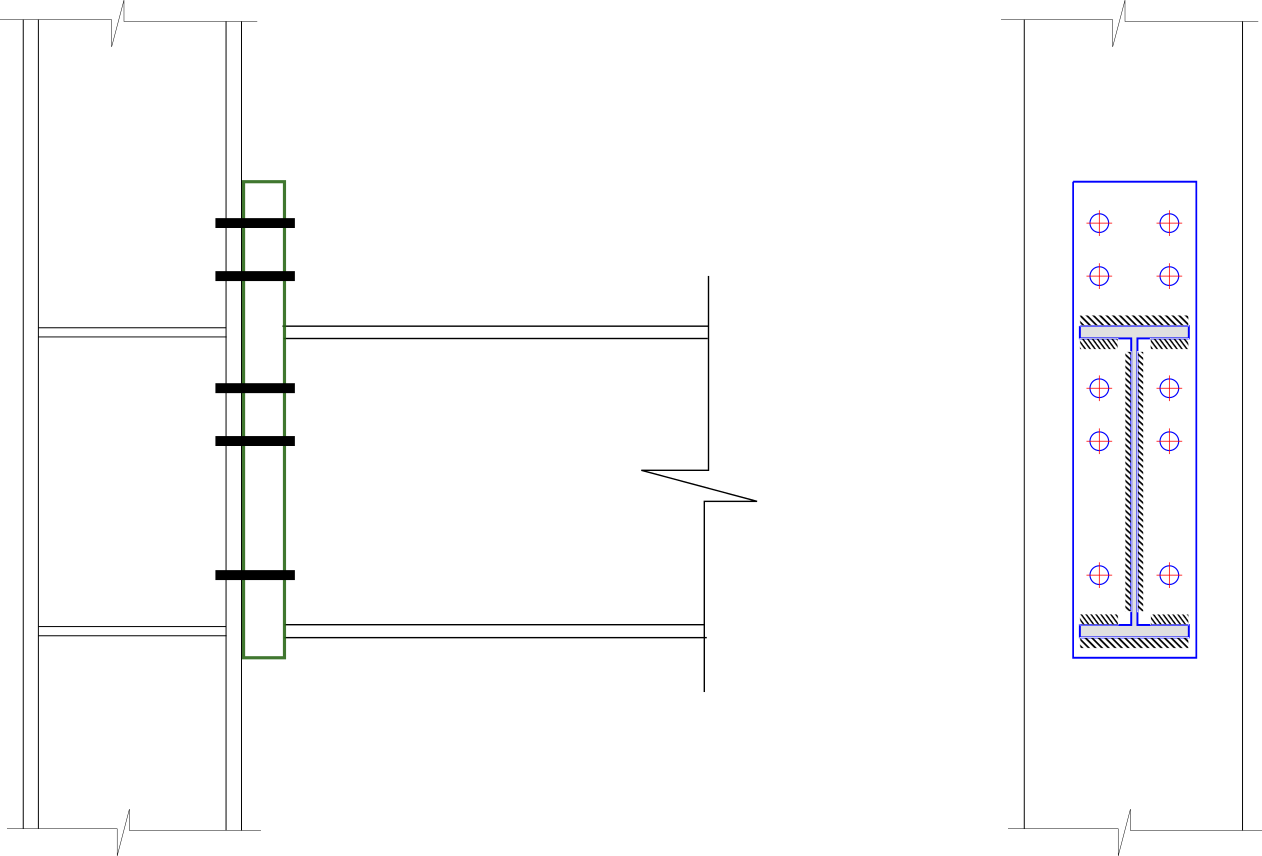
\includegraphics[height=2in]{view.png} \\	
			\vspace{3cm}
			 {\small {Prepared by:}} \\
			 {\Large \textbf {Ajmal Babu M S}} \\	
			\vspace{0.5cm}	
			{\small {Under the guidance of} }\\
			{\Large \textbf {Prof. Siddhartha Ghosh}} \\	
			\vspace{1cm}
			\centering
			
\includegraphics[width=1.2in]{logo.png} \\	
 			\vspace{0.5cm}
			{\univ} \\ 
			\vspace{0.15cm}		
			{\today}
	\end{center}
\end{titlepage}
%------------------------------------------------------
\tableofcontents
\newpage
%Print list of symbols
\printglossary[type=symbolslist,style=long]

\begin{Form}

	
\pagenumbering{arabic}	
\begin{comment}
%------------------------------------------------------

\chapter*{Guideline for filling DDCL}
	\begin{itemize}
			\item    Guideline1
			\item    Guideline2
	\end{itemize}
%------------------------------------------------------
\chapter*{Reviewer Details}
\end{comment}
%------------------------------------------------------
\chapter*{User Inputs}
%
\begin{itemize}
	\item Connecting members
		\subitem Connectivity*
		\subitem Beam Section*
		\subitem Column Section*
		\subitem $f_u$ (MPa)* 
		\subitem $f_y$ (MPa)* 
	\item Factored loads
		\subitem Moment (kNm)*
		\subitem Vert. Shear (kN)*
		\subitem Axial Force (kN)
	\item Bolt
		\subitem Diameter (mm)*
		\subitem Type *
		\subitem Grade *
	\item Plate
		\subitem Thickness (mm)*
		\subitem Height (mm)
		\subitem Width (mm)
	\item Weld size
		\subitem Flange weld (mm)*
		\subitem Web weld (mm)*
\end{itemize}
%=====================================================
\part*{Design and Detailing Checks}
%------------------------------------------------------
\chapter{Connecting Members}
%
The column and beam are allowed to connect by following connectivities.
\begin{itemize}
	\item Column flange to beam web
	\item Column web to beam web
\end{itemize}
%
\begin{comment}
The column and beam sections are provided 
as a dropdown list in Osdag input dock. 
Tapered sections from IS 808:1989 and 
parallel flange sections from the upcoming 
version of IS 808 are included. 
Old sections are highlighted in red colour 
in the dropdown with a warning that 
"user is using an old section which is not 
available in latest version of IS 808" 
in the message log.
\end{comment}
%------------------------------------------------------
%\section{Connectivity}
%------------------------------------------------------
%
\section{Column Section}
%
%All the columns sections are shown in dropdown.
%------------------------------------------------------
\section{Beam Section}
%
Currently, 
For column flange to beam web connectivity, 
\begin{equation}
	w_{fb} \le w_{fc}
\end{equation}
%
For column web to beam web connectivity,
\begin{equation}
	w_{fb} \le D_c - 2 (t_{fc} + r_{1c} + gap)
\end{equation}
Where, \\

\newgls{w_{fb}}{wfb}{Width of beam flange}
\newgls{w_{fc}}{wfc}{Width of column flange}
\newgls{D_c}{Dc}{Depth of column} 
\newgls{t_{fc}} {tfc} {Thickness of column flange} 
\newgls{r_{1c}} {r1c} {Root radius of column} or fillet size in welded sections\\
\indent $gap$ = Clearance between beam and column flanges, 5mm


%\okornot
\chapter{Material Strength}
%------------------------------------------------------
%					Material strength
%------------------------------------------------------
%
\begin{comment}
	The column, beam and end plate are supposed to have 
	the same strengths following the Indian Standards. 
	The grades available in IS 800:2007 and IS 2062:2010 
	are included with a warning that 
	"user is using a section of grade which is 
	not available in the latest version of IS 2062". 
\end{comment}
The values of material strength will be subjected to the following limits in \textbf{MPa};
\section{Yield Stress limits for beam and column}
\qquad \qquad[Reference: Table-1, IS 800 : 2007; Table-2, IS 2062 : 2011]
	\begin{equation}
		250 \leq f_{y} \leq 650
	\end{equation}
	
\section{Ultimate Stress limits for beam and column}
\qquad \qquad[Reference: Table-1, IS 800 : 2007; Table-2, IS 2062 : 2011]
	\begin{equation}
		410 \leq f_{u} \leq 780
	\end{equation}
	
\section{Yield Stress limit for end plate}
\qquad \qquad[Reference: AISC]
\begin{equation}
	f_{y} \leq 344
\end{equation}

%	\okornot

\chapter{Factored loads}
%------------------------------------------------------
%					Factored Loads
%------------------------------------------------------
%
\begin{comment}
	Factored values of the moment (in kNm) and vertical shear force  (in kN) acting on connection is mandatorily taken from the user. An optional field for axial force (in kN) is also given in the input dock if it is acting.\\
	Assuming the beam is laterally supported and factored shear force does not exceed 0.6 times its design shear strength, 
\end{comment}
	The minimum moment capacity of connection,

\section{Minimum Factored Moment} 
\qquad \qquad[Reference: Cl. 10.7, b-1, IS 800 : 2007] \\ \\
	\begin{equation}\label{eq:cl_10.7b, IS 800}
		M_{min} = 0.5 M_d 
	\end{equation}
	Where, \\
		\indent $M_{min}$ = Minimum moment capacity of the connection \\
		\indent $M_d$ = Design bending strength of the beam, given by
	\begin{equation} \label{eq:cl_8.2.1.2a, IS 800}
		M_d = \beta_b Z_p f_y / \gamma_{m0} \le 1.5 Z_e f_y / \gamma_{m0} 
	\end{equation}
	Where, \\
		\indent $\beta_b$ = 1.0 for plastic and compact sections;\\
		\indent $\beta_b$ = $Z_e/Z_p$ for semi-compact sections;\\
		
		
		\indent $Z_p, Z_e$ = Plastic and elastic section modulii of the cross-section, respectively; \\
		\indent $f_y$ = Yield stress of the material;\\
		\indent $\gamma_{m0}$ = Partial safety factor \\
		\indent $M_{min}$ = Minimum moment capacity of the connection

%\okornot

\chapter{Bolt}
%------------------------------------------------------
%					Bolt
%------------------------------------------------------
%
\begin{comment}	
	The diameter [from a dropdown list with 12, 16, 20, 24, 30 or 36 mm conforming to IS 1363 (part 1) 2002], type of bolt action (bearing or friction grip) and grade of bolts are taken from the user as inputs. The nominal tensile strength of bolt [IS 1367 (part 3): 2002] is considered as the ultimate tensile strength by default, and the user is allowed to overwrite it in 'Design Preference'. The bolt hole type is taken as 'Standard' by default and the user is allowed to change it to 'Over-sized' in 'Design Preferences,' and the bolt hole diameter is calculated accordingly, conforming to cl. 10.2.1 of IS 800:2007. The coefficient of friction (for friction grip bolts) is taken as 0.3 by default and the user is allowed to change it from a dropdown list with values given in table 20 of IS 800:2007. 
\end{comment}
%======================================================
\section{Bolt Value}
%------------------------------------------------------
\subsection{Bearing type bolts}

\subsubsection{Design strength of bolt (\boldmath $V_{db}$)}
\qquad \qquad [Reference: Cl. 10.3.2, IS 800:2007] \\ \\ 

\noindent The design strength of bolt is taken as the smaller of the value as governed by shear, $V_{dsb}$ (\ref{shear_capacity}) and bearing $V_{dpb}$ (\ref{bearing_capacity}).

\begin{equation}
	V_{db} = min~ (V_{dsb}, V_{dpb})
\end{equation}

%------------------------------------------------------
\subsubsubsection{Shear capacity (\boldmath $V_{dsb}$)}
\label{shear_capacity}
\qquad \qquad [Reference: Cl. 10.3.3, IS 800:2007] \\ \\
Currently, conservatively assuming all the shear planes passes through the threads of the bolt. Shear capacity of bearing bolts,
\begin{equation}
	V_{dsb} = \frac{f_u n_n A_{nb}}{\sqrt{3} \gamma_{mb}} \beta_{lj} \beta_{lg} 
\end{equation}
Where, \\
%\indent $V_{dsb}$ = design strength of bolt, as governed by shear strength;\\
\indent $f_u$ = ultimate tensile strength of a bolt;\\
\indent $n_n$ =  number of shear planes with threads intercepting the shear plane; \\
\indent $A_{nb}$ = net shear area of the bolt at threads, may be taken as the area corresponding to root diameter at the thread;\\
\indent $\gamma_{mb}$ = partial safety factor for bolt\\
\indent $\beta_{lj}, \beta_{lg}$ = factors, given by;

\begin{equation}
	\beta_{lj} = 1.075 - 0.005(l_j/d), 0.75 \le \beta_{lj} \le 1.0
\end{equation}

\begin{equation}
	\beta_{lg} = 8/(3 + l_g/d)
\end{equation}

Where, \\
\indent $l_J$ = length of joint (measured in the direction of load transfer); \\
\indent $l_g$ = total thickness of the connected plates (grip length); \\
\indent $d$ = nominal diameter of the bolt. \\
%------------------------------------------------------
\subsubsubsection{Bearing capacity (\boldmath $V_{dpb}$)}
\qquad \qquad [Reference: Cl. 10.3.4, IS 800:2007] \\ \\
\label{bearing_capacity}
\begin{equation}
	V_{dpb} = \frac{2.5~ k_b~ d~ t~ f_u}{\gamma_{mb}}
\end{equation}
Where, \\
\indent $k_b$ is smaller of $\frac{e}{3~d_0}, \frac{p}{3~d_0} - 0.25, \frac{f_{ub}}{f_u}, 1.0$; \\
\indent $e, p$ = end and pitch distances of the bolt along bearing direction; \\
\indent $d, d_0$ = diameter of bolt and bolt hole; \\
\indent $t$ = summation of the thicknesses of the connected plates experiencing bearing stress in the same direction; \\
\indent $\gamma_{mb}$ = partial safety factor.
%------------------------------------------------------
\subsubsection{Tension capacity (\boldmath $T_{db}$)}
\label{tension_bearing}
\qquad \qquad [Reference: Cl. 10.3.5, IS 800:2007] \\ \\
\begin{equation}
T_{db} = \frac{0.90~ f_{ub}~ A_n}{\gamma_{mb}}~ < \frac{~f_{yb}~ A_{sb}}{\gamma_{m0}}
\end{equation}
Where, \\
\indent $f_{ub}$ = ultimate tensile stress of the bolt; \\
\indent $f_{yb}$ = yield tensile stress of the bolt; \\
\indent $A_n$ = net tensile stress area of the bolt; \\
\indent $A_{sb}$ = shank area of the bolt; \\
\indent $\gamma_{mb}, \gamma_{m0}$ = partial safety factors. \\
%------------------------------------------------------
\subsection{Friction grip type bolts}
%------------------------------------------------------
\subsubsection{Slip resistance (\boldmath $V_{dsf}$)}
\qquad \qquad [Reference: Cl. 10.4.3, IS 800:2007] \\ \\
\begin{equation}
	V_{nsf} = 0.7 \mu_f n_e  K_h A_{nb} f_{ub} / \gamma_{mf}
\end{equation}
Where, \\
\indent $\mu_f$ = coefficient of friction (slip factor); \\
\indent $n_e$ = number of effective interfaces offering frictional resistance to slip; \\
\indent $K_h$ = 1.0 for bolts in clearance holes and 0.85 for bolts in oversized holes; \\
\indent $F_o$ = proof load; \\
\indent $\gamma_{mf}$ = partial safety factor.
%------------------------------------------------------
\subsubsection{Tension capacity (\boldmath $T_{df}$)}
\label{tension_friction}
\qquad \qquad [Reference: Cl. 10.4.5, IS 800:2007] \\ \\
\begin{equation}
T_{df} = \frac{0.9~ f_{ub}~ A_n}{\gamma_{mf}} ~\leq~ f_{yb} A_{sb}  \frac{\gamma_{m1}}{\gamma_{m0} \gamma_{mf}}
\end{equation}
Where, \\
\indent $f_{ub}$ = ultimate tensile stress of the bolt; \\
\indent $f_{yb}$ = yield tensile stress of the bolt; \\
\indent $A_n$ = net tensile stress area of the bolt; \\
\indent $A_{sb}$ = shank area of the bolt; \\
\indent $\gamma_{m1}, \gamma_{mf}$ = partial safety factors. \\

%======================================================
%------------------------------------------------------
%======================================================
\section{Minimum Number of bolts}
%------------------------------------------------------
Minimum number of bolts required is calculated based on the tension acting on bolts. A 20~\% reduction on bolt tensile capacity is assumed to account the prying force. Total number of bolts in the configuration is determined based on the layouts given in Sec. \ref{layout} \\
Minimum number of bolts required at the tension side, $n_f$

\begin{equation}
	n_f = \frac{T_f}{0.8 * T_b}
\end{equation}

Where, \\
\indent $T_b$ = tension capacity of bolts \\
\indent $T_f$ = tension in flange, calculated as; \\

\begin{equation}
	T_{f} = \frac{M_u}{D - t_f} ~ + ~ \frac{H}{2}
\end{equation}

Where, \\
\indent $M_u$ = factored bending moment acting on the connection. \\
\indent $D$ = depth of the beam; \\
\indent $t_f$ = thickness of the beam flange; \\
\indent $H$ = axial force acting on the connection. \\


\section{Layout of Bolts}
\label{layout}
\subsection{Flush end plate}
	\begin{multicols}{2}
		\begin{center}
			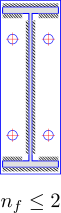
\includegraphics{bolt_layout1.png}
		\end{center}
		\begin{center}
			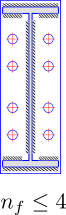
\includegraphics{bolt_layout2.png}
		\end{center}
	\end{multicols}
\clearpage
\subsection{Extended one way end plate}
	\begin{multicols}{3}
		\begin{center}
			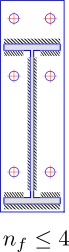
\includegraphics{bolt_layout3.png}
		\end{center}
		\begin{center}
			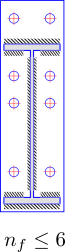
\includegraphics{bolt_layout4.png}
		\end{center}
		\begin{center}
			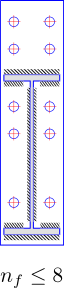
\includegraphics{bolt_layout5.png}
		\end{center}
	\end{multicols}

\subsection{Extended both ways end plate}
	\begin{multicols}{3}
		\begin{center}
			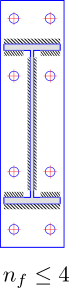
\includegraphics{bolt_layout7.png}
		\end{center}
		\begin{center}
			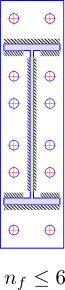
\includegraphics{bolt_layout8.png}
		\end{center}
		\begin{center}
			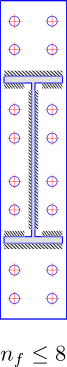
\includegraphics{bolt_layout9.png}
		\end{center}
	\end{multicols}

\section{Tension in bolts}
\subsection{Tension due to applied axial force}
\quad \quad[Reference: Cl. 10.11.2.1(a), IS 800:2007] \\ \\
The applied axial force is considered to be equally shared by the bolts. The tension in bolts due to applied axial force ($T_{ix}$) is calculated as 
\begin{equation}
T_{ix} = F_x / n  
\end{equation}
Where, \\
\noindent $F_x$ = applied axial force, \\
\noindent $n$ = Total number of bolts in the configuration \\
\subsection{Tension due to applied moment}
\quad \quad[Reference: Cl. 10.11.2.1(b), IS 800:2007] \\ \\
The tension due to applied moment ($T_{im}$) is considered to vary linearly with the distance from the relevant neutral axis. As column stiffeners are providing, the end plate connection can be assumed as pivoting about the bottom (compression) flange and the neutral axis can be assumed as the mid depth of bottom compression flange.

\begin{figure}[h]
	\centering
	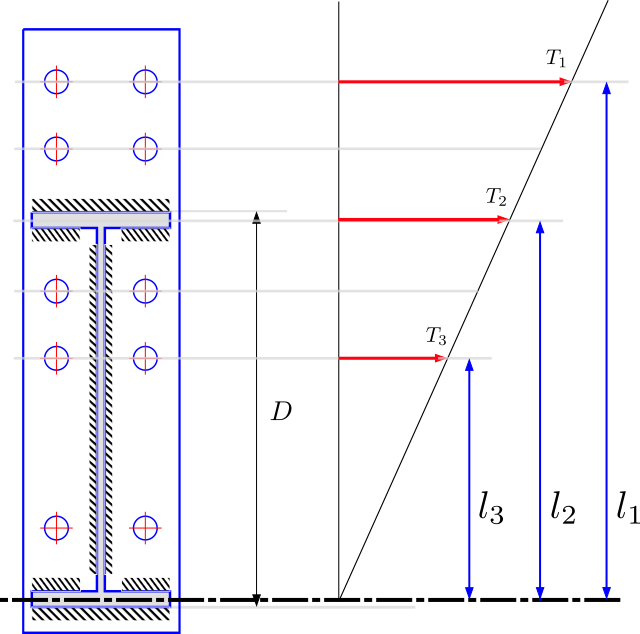
\includegraphics[width=0.3\linewidth]{tension.png}
	\caption{Linear distribution of tensile forces in bolts}
	\label{fig: tensile_distribution}
\end{figure}

The nominal tensile forces in the bolts ($T_{im}$) are calculated assuming it to be proportional to the distance of the bolt from the neutral axis ($l_i$) as in Fig.~\ref{fig: tensile_distribution}. For calculating the bolt tensions in the rows immediately above and below the tension flange, $l_i$ is taken as the distance of the tension flange from the neutral axis as the top portion of the plate behaves as a T- stub, symmetric about the tension flange. Tension in bolts near to the compression flange can be neglected. [INSDAG Teaching Materials, Narayanan, et al., 2001, DoSS, N.Subramanian, 2014]. 

\begin{equation}
	T_{im} = k * l_i 
\end{equation}
where $k$ is a constant\\
Moment acting on the connection due to applied moment, 
\begin{equation}
	M =  \sum T_{im} * l_i  = k \sum {l_i}^2
\end{equation}

\begin{equation}
	T_{im} = \frac {M l_i} {\sum {l_i}^2}
\end{equation}
\subsection{Prying force in bolts}
\quad \quad[Reference: Cl. 10.4.7, IS 800:2007] \\

\begin{equation}
	Q = \frac{l_v}{2~l_e} \bigg [T_e - \frac{\beta~ \eta~ f_o~b_e~t^{4}}{27~ l_e~l_v^{2}} \bigg]
\end{equation}

Where, \\
\indent $l_v$ = distance from the bolt centreline to the toe of the fillet weld or to half the root radius for a rolled section;\\
\indent $l_e$ = distance between prying force and bolt centreline, and, is given by;

\begin{equation}
	l_e = minimum~ \Bigg(e,~1.1~t~ \sqrt{\frac{\beta~f_o}{f_y}}~ \Bigg)
\end{equation}

\indent $e$ = end distance; \\
\indent $\beta$ = 2 for non pre-tensioned bolt and 1 for pre-tensioned bolt; \\
\indent $\eta$ = 1.5; \\
\indent $b_e$ = effective width of flange per pair of bolts; \\
\indent $f_o$ = proof stress, and; \\
\indent $t$ = thickness of the end plate. \\


\subsection{Check for total tension in bolts}


Tension in critical bolt(s) due to applied loads and prying forces is checked against the tension capacity ($T_d$) of bolt defined in Sec. \ref{tension_bearing} and Sec. \ref{tension_friction} \\

\begin{equation}
	T_{cx} + T_{cm} + Q \le T_d
\end{equation}

Where, \\
\indent $T_{cx}$ = tension in critical bolt due to applied axial force \\
\indent $T_{cm}$ = tension in critical bolt due to applied moment \\
\indent $Q$ = prying force acting on critical bolt \\

%---------------------------------------------------------------------		
\section{Combined shear and tension in bolts}
\subsection{For friction grip bolt(s)}
\qquad \qquad [Reference: Cl. 10.4.6, IS 800:2007] \\ \\

\begin{equation}
	\bigg(\frac{V_{sf}}{V_{df}}\bigg)^{2} ~ + ~ \bigg(\frac{T_{f}}{T_{df}}\bigg)^{2} ~ \leq ~ 1.0
\end{equation}

Where, \\
\indent $V_{sf}$ = applied factored shear at design load; \\
\indent $V_{df}$ = design shear strength of bolt; \\
\indent $T_f$ = externally applied factored tension at design load, and; \\
\indent $T_{df}$ = design tension strength of bolt; \\


\subsection{For bearing bolt(s)}
\qquad \qquad [Reference: Cl. 10.3.6, IS 800:2007] \\ \\

\begin{equation}
	\bigg(\frac{V_{sb}}{V_{db}}\bigg)^{2} ~ + ~ \bigg(\frac{T_{b}}{T_{db}}\bigg)^{2} ~ \leq ~ 1.0
\end{equation}

Where, \\
\indent $V_{sb}$ = factored shear force acting on the bolt; \\
\indent $V_{db}$ = design shear capacity of bolt; \\
\indent $T_b$ = factored tensile force acting on the bolt, and; \\
\indent $T_{db}$ = design tension capacity of bolt; \\

%\okornot


	
\chapter{Detailing}
%------------------------------------------------------
%					Detailing
%------------------------------------------------------	
	\begin{figure}[h]
		\centering
		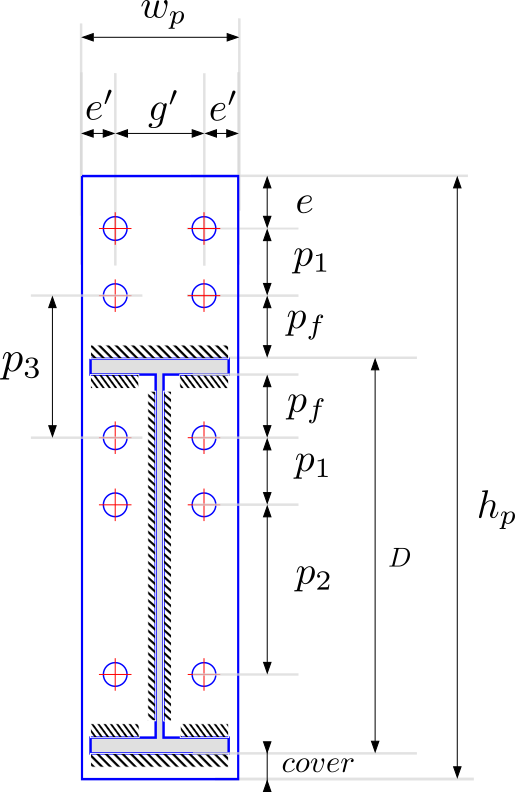
\includegraphics[width=4in]{detailing.png}
		\caption{detailing}
	\end{figure}

\section{Pitch (p) and gauge (g) distances}
	Pitch (p) is the distance between centres of two adjacent fasteners in a line lying in the direction of stress.
	Gauge (g) is the distance between centres of two adjacent fasteners transverse to the direction of stress.

\subsection{Minimum pitch (p) and gauge distances}
	\qquad \qquad [Reference: Cl. 10.2.2, IS 800 : 2007]\\
		\begin{equation}
			 pitch (p)/gauge (g) \ge 2.5 * bolt\, diameter
		\end{equation}
				
\subsection{Maximum pitch (p) and gauge distances}
\qquad \qquad [Reference: Cl. 10.2.3, IS 800 : 2007]\\				
		\begin{equation}
			pitch (p)/gauge (g) \leq min(32 * t,\, 300\, mm)
		\end{equation}
		where, \\
			\indent t = thickness of thicker plate being connected 

\section{End (e) and edge (e') distances}
				
\qquad \qquad [Reference: Clause 10.2.4.1, IS 800 : 2007] \\
 
The edge distance (e') is the distance at right angles to the direction of stress from the centre of a hole to the adjacent edge. The end distance (e) is the distance in the direction of stress from the centre of a hole to the end of the element.

\subsection{Minimum end (e) and edge (e') distances}
\qquad \qquad [Reference: Cl. 10.2.4.2, IS 800 : 2007]\\

For sheared or hand-flame cut edges;
	\begin{equation}
		{end (e)/edge (e')} ~ \geq ~ 1.7 * d_0
	\end{equation}

For rolled, machine-flame cut, sawn and planed edges;
	\begin{equation}
		{end (e)/edge (e')} ~ \geq ~ 1.5 * d_0
	\end{equation}
	
Where $d_0$ is the diameter of bolt hole

\subsection{Maximum end (e) and edge (e') distances}
\qquad \qquad [Reference: Cl. 10.2.4.3, IS 800 : 2007]\\

\begin{equation}
{end (e)/edge (e')} ~ \leq ~ 12  t  \varepsilon
\end{equation}			

	\begin{equation}
		\varepsilon = \sqrt{\frac{250}{f_y}}
	\end{equation}
	
	Where, \\
	\indent $d_0$ = diameter of the hole; \\
	\indent $t$ = thickness of the thinner plate; \\
	\indent $f_y$ = yield stress of the plate.

				
\section{Cross-centre gauge distance (g')} 
Cross centre gauge is the distance between immediate columns of bolts on either side of beam web.

		\subsection{Flush end plate}
		\qquad \qquad [Reference: AISC Design Guide - 16, table 3-6, page 22]
		\begin{equation}
		 	57 mm \leq \textbf{g'} \leq 95 mm 
		\end{equation}
		
		\subsection{Extended one way}
		\qquad \qquad [Reference: AISC Design Guide - 16, table 4-7, page 39]
		\begin{equation}
			 69 mm \leq \textbf{g'} \leq 177 mm
		\end{equation}

\section{Distance between centre of bolt and edge of the beam flange ($p_{f}$)}
	
		\subsection{Flush end plate}
		\qquad \qquad [Reference: AISC Design Guide - 16, table 3-6, page 22]
			\begin{equation}
				33 mm \leq p_{f} \leq 47 mm
			\end{equation}
			
		\subsection{Extended one way}
		\qquad \qquad [Reference: AISC Design Guide - 16, table 4-7, page 39]
			\begin{equation}
				25 mm \leq p_{f} \leq 38 mm
			\end{equation}

\section{Projection of plate beyond the flanges ($c$)}
\label{projection}
This specifies the projection of end plate beyond the bottom and top flanges of beam in flush end plate connection and bottom flange of beam in one way extended end plate connection.


\chapter{End Plate} 
%------------------------------------------------------
%					End Plate
%------------------------------------------------------	
\section{Plate height \boldmath $(h_{p})$}
	\subsection{Minimum plate height}
	\qquad \qquad [Reference: based on detailing] \\ \\
	\subsubsection{for flush end plate}
		\begin{equation}
			h_p \ge D + 2 * (t_{wf} + projection)
		\end{equation}
	
	\subsubsection{for extended one way end plate}
	\begin{equation}
	h_p \ge D + (2 * t_{wf}) + p_f + e + projection
	\end{equation}
	
	\subsubsection{for extended both ways end plate}
	\begin{equation}
	h_p \ge D + 2 * (t_{wf} + n'*p + p_f + e + projection)
	\end{equation}
				
		Where, \\
	\indent $D$ = depth of beam; \\
	\indent $t_{wf}$ = size of weld at flange; \\
	\indent $p_f$ =  distance between centre of the bolt and toe of weld at flange;\\
	\indent $e$ = end distance; \\
	\indent $projection$ = as per \ref{projection}\\
	\indent $n'$ = number of rows of bolts beyond the flange

\section{Plate Width (\boldmath $w_p$)}
\qquad \qquad [Reference: based on detailing] \\
	\begin{equation}
		w_p = g' + (2 * e')
	\end{equation}

\subsection{Minimum plate width (\boldmath $w_{p_{min}}$)} 
\qquad \qquad [Reference: based on detailing] \\
	\begin{equation}
		w_{p_{min}} = b_f
	\end{equation}

\subsection{Maximum plate width (\boldmath $w_{p_{max}}$)}
\qquad \qquad [Reference: AISC Design Guide - 16] \\
	\begin{equation}
		w_{p_{max}} = b_f + 25~mm
	\end{equation}
			


\section{Plate thickness $(t_{p})$}
\begin{figure}[h]
	\centering
	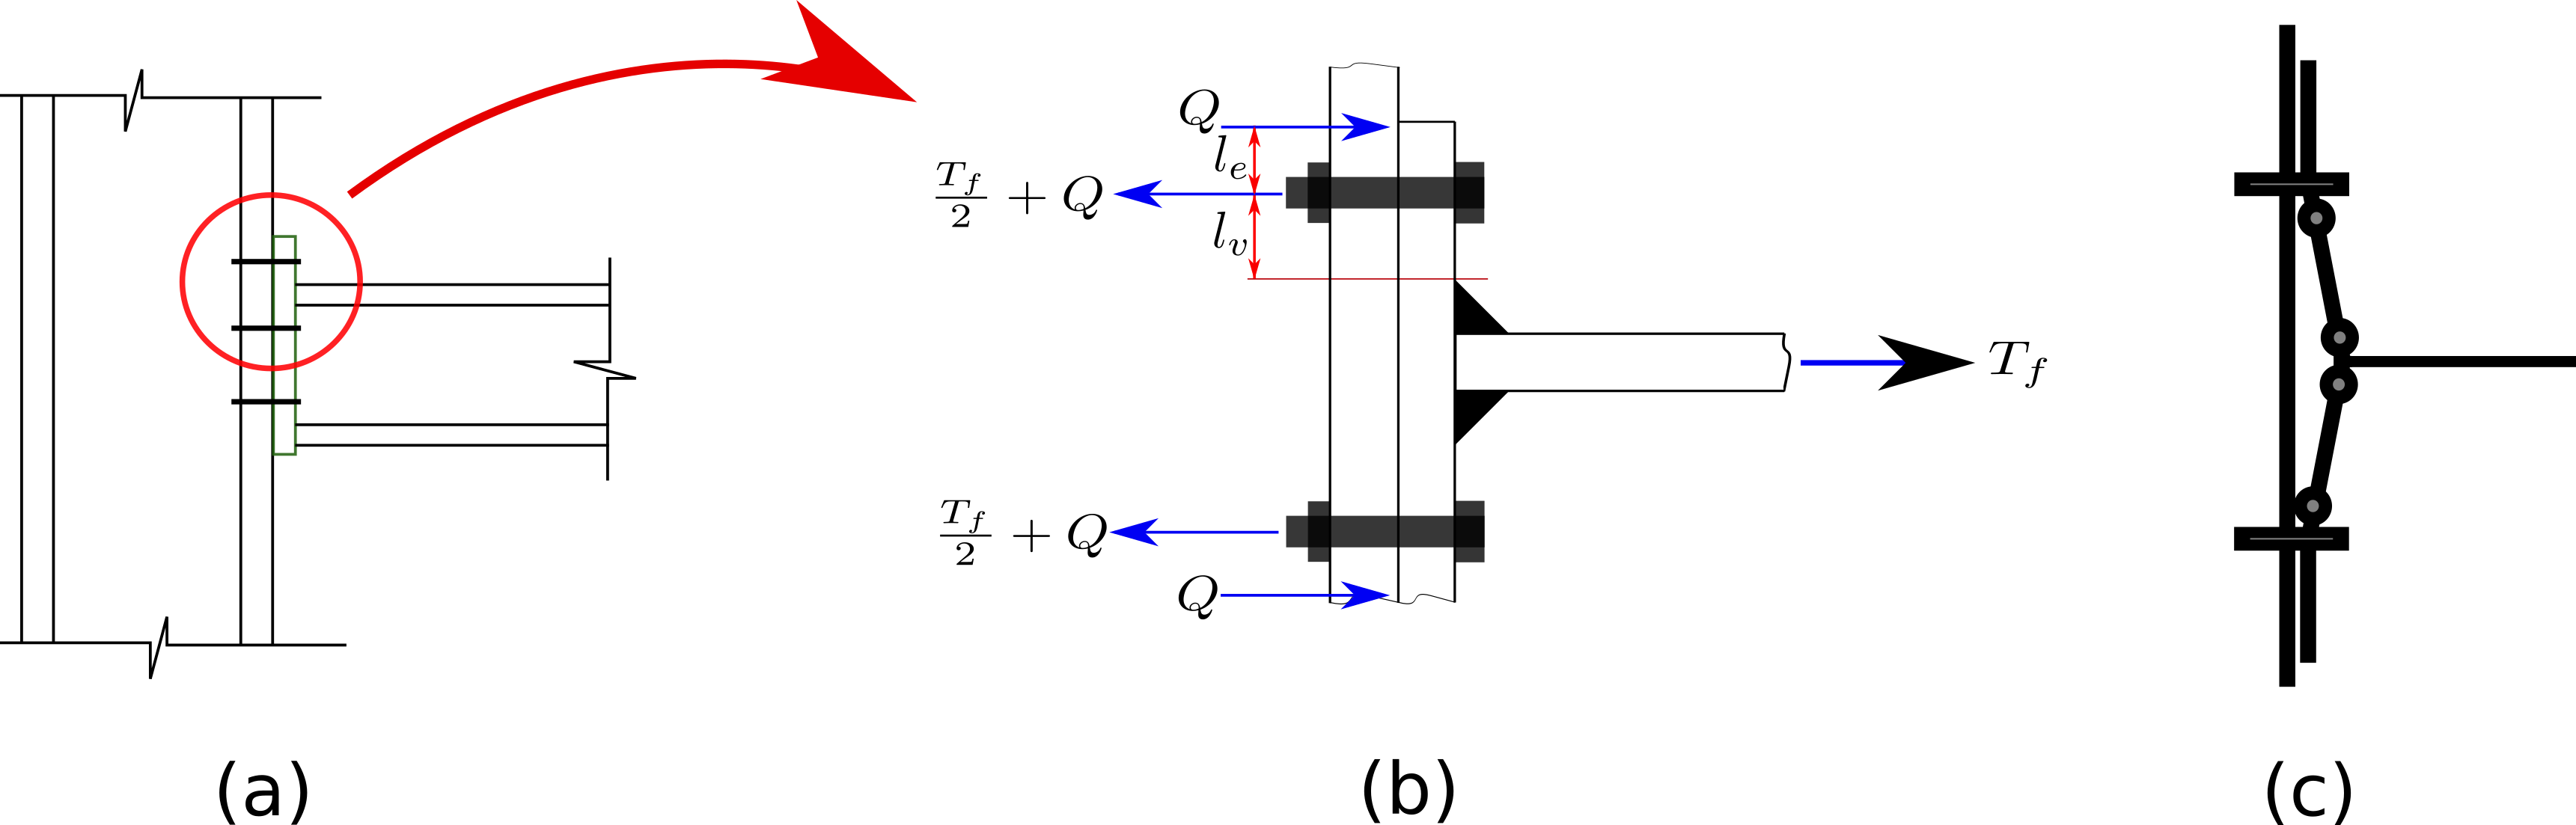
\includegraphics[width=0.8\linewidth]{prying.png}
	\caption{Prying force}
	\label{fig:prying}
\end{figure}


The required minimum thickness of plate is determined from it's plastic moment capacity~($M_p$), equated to the moment at toe of weld~($M$). The tension in flange ($T_f$) will induce prying force in bolts (Q). As the tension in flange increases, the portion of the end plate near the toe of weld will begin to separate from the connected member by forming a plastic hinge. Thus, this portion of the end plate (indicated by `A' in \ref{fig:prying}) is the critical section.\\


\textbf{Moment at toe of weld} \\
	\begin{equation}
		M = \frac{T_f}{2}  l_v ~ - ~ Q ~ l_e
	\end{equation}

\textbf{Plastic Moment $M$ with $M_p$} \\
	\begin{equation}
		M_p = \bigg(\frac{f_y}{1.10}\bigg) ~ \bigg(\frac{b_e~t_{p}^{2}}{4}\bigg)
	\end{equation}
	
\textbf{The required thickness of end plate ($t_{p,required}$)} \\

	\begin{equation}
		t_{p,required} = \sqrt{M~ \bigg(\frac{1.10}{f_y}\bigg) ~ \bigg(\frac{4}{b_e}\bigg)}
	\end{equation}
	Where, \\
\indent $f_y$ = yield strength of plate; \\
\indent $b_e$ = effective width of end plate per pair of bolt ($\frac{w_p}{2}$, for 2 columns of bolt).


\chapter{Weld}
%------------------------------------------------------
%					Weld
%------------------------------------------------------	 

\begin{figure}[h]
	\centering
	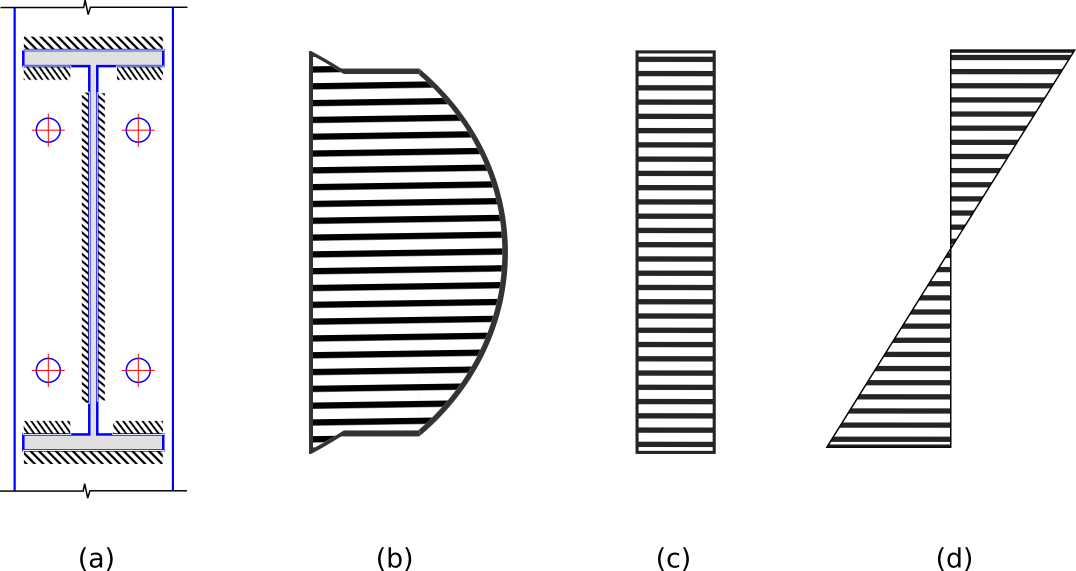
\includegraphics[width=0.7\linewidth]{weld_stress.png} \\
	{(a) Welding in the end plate connection, (b) Actual shear stress distribution, (c) Assumed shear stress distribution, (d) Actual bending moment distribution, (e) Assumed bending moment distribution}
	\caption[Weld stress]{Weld profile}
	\label{fig:weld_stress}
\end{figure}

In a beam to column end plate moment connection, the beam is welded to the end plate as shown in figure~\ref{fig:weld_stress}~(a). Since the locations of maximum bending and shearing stresses are not same (figure~\ref{fig:weld_stress}~b and d), it can be safely assumed that the web welds would carry the entire shear force and the flange welds would carry entire bending moment [Ref: DoSS, N. Subramanian] 

\section{Weld size}

\subsection{Minimum weld size}
\quad \quad [Reference: Table 21, IS 800:2007] \\

\begin{figure}
	\centering
	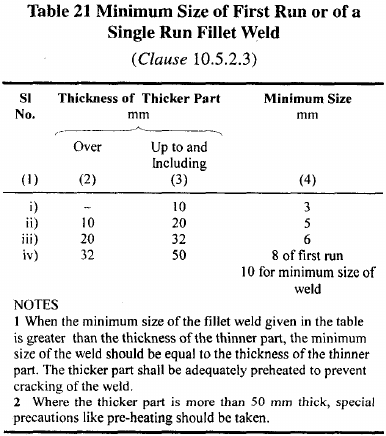
\includegraphics[width=0.3\linewidth]{min_weld}
	\caption{Minimum Size of First Run or of a Single Run Fillet Weld}
	\label{fig:minweld}
\end{figure}

\subsection{Maximum weld size}
\quad \quad [Reference: Cl. 10.5.3, IS 800:2007] \\

The maximum size of weld = Thickness of thinner element being welded. \\


\subsection{Throat size of weld}
\quad \quad [Reference: Cl. 10.5.3.2, IS 800:2007] \\
Throat size of weld, 
\begin{equation}
	t_t = 0.70 * z
\end{equation}


\section{Weld lengths}
As a smaller size of weld will be economical than a larger one for the same strength, maximum possible lengths are provided on flanges and web of beam as shown in figure~\ref{fig:weldlength}.
\begin{figure}[h]
	\centering
	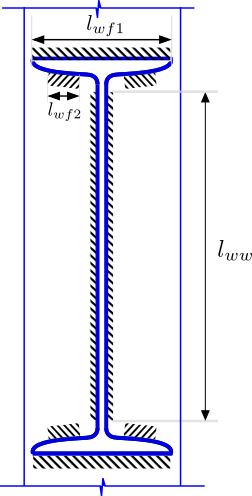
\includegraphics[width=0.2\linewidth]{weld_length}
	\caption{Flange and web welds}
	\label{fig:weldlength}
\end{figure}

\subsection{Length of flange welds}

Welds are given in above and below of flanges. \\
The length of weld above the flange, 
\begin{equation}
	l_{wf1} = w
\end{equation}

The length of weld below the flange, 
\begin{equation}
	l_{wf2} = \frac{w- t_w - 2~r_1 - 2~r_2 }{2} \nless 4~z_f
\end{equation}

Where, \\
\indent $w$ = width of flange, \\
\indent $t_w$ = thickness of beam web, \\
\indent $r_1$ = root radius of beam, \\
\indent $r_2$ = toe radius of beam, \\

Effective lengths of welds at flange, \\
\begin{equation}
	l_{wf1,eff} = l_{wf1} - 2~z_f
\end{equation}
\begin{equation}
	l_{wf2,eff} = l_{wf2} - 2~z_f 
\end{equation}


The total effective length of welds at flange, \\

\begin{equation}
	l_{wf,eff} = l_{wf1,eff} + 2~l_{wf2,eff}
\end{equation}

%\begin{equation}
%	 = 2~w - t_w - 2~r_1 - 2~r_2 - 6~z_f 
%\end{equation}

\subsection{Length of web welds}
Welds are given on both flat sides of beam web (marked as $h_1$ in \textit{SP 6-1: ISI Handbook for Structural Engineers -Part-~1 Structural Steel Sections, BIS, 1964}). \\

The flat web length can be computed as, 
\begin{equation}
	l_{ww} = d- 2(t_f + \frac{B-t_w}{2}~\tan (\alpha-\pi/\small{2} + r_1)
\end{equation}

The effective length of welds at either side of beam web, \\

\begin{equation}
	l_{ww,eff} = l_{ww}-2~z_w
\end{equation}


\subsection{Check for long joint of weld}
Reduction for long joints in weld groups are applied as,
if $l_w > 150~t_t$,

\begin{equation}
	\beta_{lw}=1.2-\frac{0.2~l_j}{150~t_t} \le 1.0
\end{equation}


\section{Shear stresses in welds}

\subsection{Design shear strength of fillet weld}
\quad \quad [Reference: Cl. 10.5.7.1.1, IS 800:2007] \\

\begin{equation}
	f_{wd} = \beta_{lw} \frac{f_u}{\sqrt{3}~\gamma_{mw}}
\end{equation}
where, \\
\indent $f_u$ = smaller of the ultimate stress of the weld or of the parent metal, \\
\indent $\gamma_{mw}$ = partial safety factor, 1.25 for shop weld and 1.50 for field weld, \\
\indent $\beta_{lw}$ = reduction factor for long joint, if applicable. \\

\subsection{Design forces at welds due to loads}

\subsubsection{Design force on welds due to applied axial load}
\quad \quad[Reference: Cl. 10.11.2.1(a), IS 800:2007] \\ \\
The applied axial force is considered to be equally shared by the weld group.
The design shear force on unit length of fillet weld group due to axial force,
\begin{equation}
	F_{wx} = \frac{F_x}{2(l_{ww,eff} + l_{wf,eff})}
\end{equation}

\subsubsection{Design stress on welds due to applied moment}

The moment is transferred through beam flanges in the form of tension and compression.
%The design bending stress on either of flanges due to the applied moment,
%\begin{equation}
%	f_b = M/Z
%\end{equation}
The design tension/compression on either of beam flanges due to applied moment,
\begin{equation}
	T_{f} = \frac{M_u}{D - t_f}
\end{equation}
The design shear force on unit length of fillet weld group (at flanges) due to applied moment,

\begin{equation}
	F_{wt} = \frac{T_{f}}{l_{wf,eff}}
\end{equation}

\subsubsection{Design stress on welds due to applied vertical shear}
The shear force acting at the connection can be assumed as transfers to web welds only. (Refer fig.~\ref{fig:weld_stress}).
The design shear force on unit length of fillet weld group (at web) due to applied vertical shear force,

\begin{equation}
	F_{wv} = \frac{V}{2~l_{ww,eff}}
\end{equation}


\subsection{Design stresses at welds due to loads}

The flange welds possess shear stresses due to applied moment and applied axial force.
The web welds posses shear stresses due to applied shear force and applied axial force.

\subsubsection{Shear stress at flange welds}
The total shear stress at flange welds due to applied moment (in the form of tension/compression)
and applied axial force,


\begin{equation}
	f_{wf} = \frac{F_{wx} + F_{wt}}{0.7~z_f} \leq f_{wd}
\end{equation}

\subsubsection{Compression stress check at flange weld}
To be discussed

\subsubsection{Shear stress at web welds}
The applied shear force acts in vertically downward and 
applied axial force acts in the longitudinal direction of beam,
which are orthogonal. 
The resultant shear stress acting on web welds,

\begin{equation}
	f_{ww} = \frac{\sqrt{{F_{ww}}^2 + {F_{wx}}^2}}{0.7~z_w} \leq f_{wd}
\end{equation}

\chapter{Local check of Member elements, Continuity Plates and Stiffeners}
%------------------------------------------------------
%				Local check of Member elements, Continuity Plates and Stiffeners
%------------------------------------------------------	 

\section{Horizontal Continuity Plate in compression region}
The horizontal Continuity Plate in compression region is provided to counteract the beam flange compressive force, 
\begin{equation}
	P_{bf} = \frac{M_u}{D_b - t_{fb}} - F_x
\end{equation}
where,\\
\indent $P_{bf}$ = compressive force at beam flange \\ 
\indent ${M_u}$ = applied bending moment \\ 
\indent $D_b$ = depth of beam \\
\indent $t_{fb}$ = thickness of beam flange \\
\indent $F_x$ = applied factored axial tensile force in the beam flange\\

\noindent
Continuity Plates are provided if,
\begin{equation}
	P_{bf} >  R_{wc}
\end{equation}
\noindent
where,
\begin{equation}
	R_{wc} = max(R_{wcy}, R_{wcb}, R_{wcr})
\end{equation}

\newgls{R_{wc}}{Rwc}{Capacity of column web}
\newgls{R_{wcy}}{Rwcy}{Capacity of column web against local yielding}
\newgls{R_{wcb}}{Rwcb}{Capacity of column web against compression buckling}
\newgls{R_{wcr}}{Rwcr}{Capacity of column web against crippling}
\\
Continuity Plates are provided on either side of column web for full depth of column and width of flange.
The dimensions of column web stiffeners will be, \\
\begin{equation}
	length = l_{stC} = D_c-2~t_{fc}
\end{equation}
\begin{equation}
	width = w_{stC} = \frac{w_{fc}-t_{wc}}{2}
\end{equation}
\begin{equation}
	thickness = t_{stC} \ge max(\frac {l_{st}} {9.4 \epsilon_{st}} ,
	\frac{P_{bf}-R_{wc}}{f_{yst}/\gamma_{m0}} )
\end{equation}
where, 
\begin{equation}
	\epsilon_{st} = \sqrt{\frac{250}{f_{yst}}}
\end{equation}


\subsection{Local web yielding}
\qquad \qquad[Reference: DoSS, N.Subramanian, pp504] \\ \\
Capacity of column web at the toe of flange-to-web fillet against local yielding,
(Assuming a load dispersion of 2.5 to 1 slope as per IS~800:2007, Cl. 8.7.4).

\begin{equation}
	R_{wcy} = t_{wc}(5~t_{fc} + 5~r_{1c} + t_{fb}) \frac{f_{yw}}{\gamma_{m0}}
\end{equation}


\subsection{Compression buckling of web}
\qquad \qquad[Reference: DoSS, N.Subramanian, pp505] \\ \\
\noindent
Capacity of column web against compression buckling,
\begin{equation}
	R_{wcb} = 10710~({t_{wc}}^3 /h) \sqrt{(f_{yw}/ \gamma_{m0})}
\end{equation}


\subsection{Web crippling}
\qquad \qquad[Reference: DoSS, N.Subramanian, pp505] \\ \\
\noindent
Capacity of column web against crippling,
\begin{equation}
	R_{wcr} = (\frac{300~ {t_{wc}}^2}{\gamma_{m1}})
	[1+3~\frac{t_{fb}}{D_c} ~ {\big{(}\frac{t_{wc}}{t_{fc}}\big{)}}^{1.5}]
	\sqrt{\frac{f_{yw} t_{fc}}{t_{wc}}}
\end{equation}



\section{Continuity Plates in tension region}
\qquad \qquad[Reference: DoSS, N.Subramanian, pp506] \\ \\
\noindent
The continuity plates in tension region is provided to counteract the beam flange tension, 
\begin{equation}
	T_{bf} = \frac{M_u}{D_b - t_{fb}} + F_x
\end{equation}

\noindent
Nominal strength of column flange, 
\begin{equation}
	P_n = \frac{{t_{fc}}^2}{0.16} \frac{f_{yf}}{\gamma_{m0}}	
\end{equation}

\noindent
Continuity plates are provided if,
\begin{equation}
	T_{bf} >  P_n
\end{equation}

\noindent
Tension continuity plates are provided on either side of column web for full depth of column and width of flange.
The dimensions of Continuity plates will be, \\
\begin{equation}
	length = l_{stT} = D_c-2~t_{fc}
\end{equation}
\begin{equation}
	width = w_{stT} = \frac{w_{fc}-t_{wc}}{2}
\end{equation}
\begin{equation}
	thickness = t_{stT} \ge \frac{T_{bf}-P_n}{f_{yst}/\gamma_{m0}}
\end{equation}



\section{Diagonal Stiffener}
\qquad \qquad[Reference: DoSS, N.Subramanian, pp 503,507] \\ \\
\noindent
Diagonal stiffeners are provided to resist the large shear produced by the applied moment at the portion of column web in connection. 

\noindent
Diagonal stiffeners are provided if,
\begin{equation}
	t_{wc} > \frac{1.9 M_u}{D_b D_c f_{ywc}}
\end{equation}
\noindent
Area of stiffener required, 
\begin{equation}
	A_{stD} = 
	\frac{\gamma_{m0}}{f_y \cos{\theta}} ~ [
	\frac{M}{D_b} - 
	\frac{f_y t_{wc} D_c}{\sqrt{3} ~ \gamma_{m0}} ]
\end{equation}
where,
\begin{equation}
	\cos{\theta} = \frac{D_c - 2 t_{fc}}
	{\sqrt{{{(D_c - 2 t_{fc})}^2 + (D_b - 2 t_{fb})}^2}}
\end{equation}


\section{Local check of beam flange against yielding}
The developed force in the beam flange = force transferred to the horizontal stiffeners = $P_{bf}$ or $T_{bf}$.\\
\\
\\
\indent $b_{bf}$ = width of beam flange \\ 
\indent $t_{bf}$ = thickness of beam flange \\
\newgls{P_{loc,bf}}{P_{loc}}{Local capacity of beam flange}\\
\\
Local capacity of beam flange,
\begin{equation}
	P_{loc,bf} = \frac{b_{bf} t_{bf} f_y}{\gamma_{m0}}
\end{equation}
\\
Check,\\
\begin{equation}
	P_{loc,bf} \geq P_{bf}\:or\:T_{bf}
\end{equation}


%\pagebreak
\section{Weld size of column web continuity plates}

\begin{figure}[ht]
	\centering
	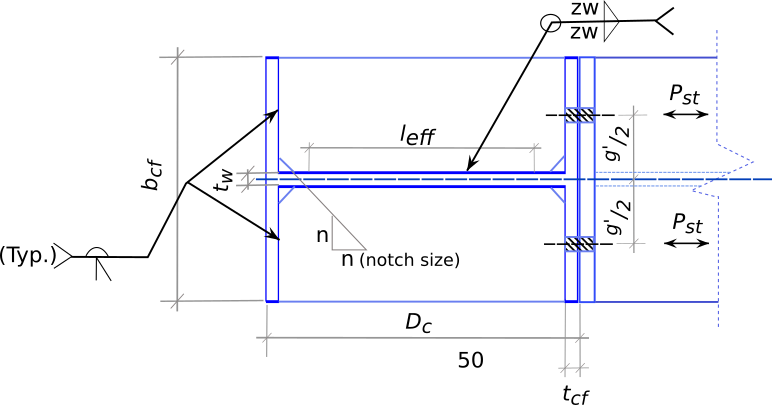
\includegraphics[scale=0.5]{COLCP.png}
\end{figure}

\noindent
Force induced in each piece of the column continuity plate = $P_{bf}/2$ \: or \: $T_{bf}/2$.\\
\\
Moment induced in the column continuity plate = $ \frac{P_{bf}} {2}  \frac{g'} {2} $ \: or \: $ \frac{T_{bf}} {2}  \frac{g'} {2} $\\
\\
\indent $g'$ = gauge of the end plate bolts \\ 
\\
\noindent
To transfer the force from the column flange to the continuity plates, it is preferable that the continuity plates are butt welded to the column flanges.
\\
The fillet weld between the continuity plates and the column web need to be checked for the force transferred through the continuity plates i.e. $P_{bf}/2$ \: or \: $T_{bf}/2$.\\
\\
Effective length of the continuity plate, $l_{eff} = ( D_c - 2t_{cf} - 2n )$ \\
Total length of weld available, $l_w = 2(\, l_{eff} - 2.w)$ \\
\\
\indent $D_c$ = depth of column \\ 
\indent $t_{cf}$ = thickness of column flange \\
\indent $n$ = notch size \\
\indent $w$ = weld size \\
\\
Capacity of fillet weld,
\begin{equation}
	P_w = \frac{l_w . f_u . w_{tt}}{\sqrt{3} \gamma_{mw}}\\
\end{equation}
\\
\indent $w_{tt}$ = throat thickness of fillet weld \\
\\
The moment in the continuity plate, due to eccentricity of force can be taken care of by the weld between the continuity plate and the column flange. Since this is a butt weld, we need to check shear capacity of the continuity plate in this direction only.
\\
Shear force in this direction = $ \frac{P_{bf} \: e}{2 d_{st}} $ \: or \: $ \frac{T_{bf} \: e} {2 d_{st}} $\\
\\
Shear capacity of the continuity plate plate, $V_{st} = \frac{b_{st,eff} t_{st} . f_y}{\sqrt{3} \gamma_{m0}}$\\
\\
\indent $d_{st}$ = depth of continuity plate = $D_c - 2t_{cf}$ \\
\indent $b_{st,eff}$ = width of continuity plate = $(b_{cf} - t_w)/2 - n$ \\
\indent $t_{st}$ = thickness of continuity plate \\


\section{End Plate Stiffeners}
Considering that moment developed at the beam column junction is clockwise in nature, the top stiffener will be under shear and bending moment as shown in the following figure.\\

%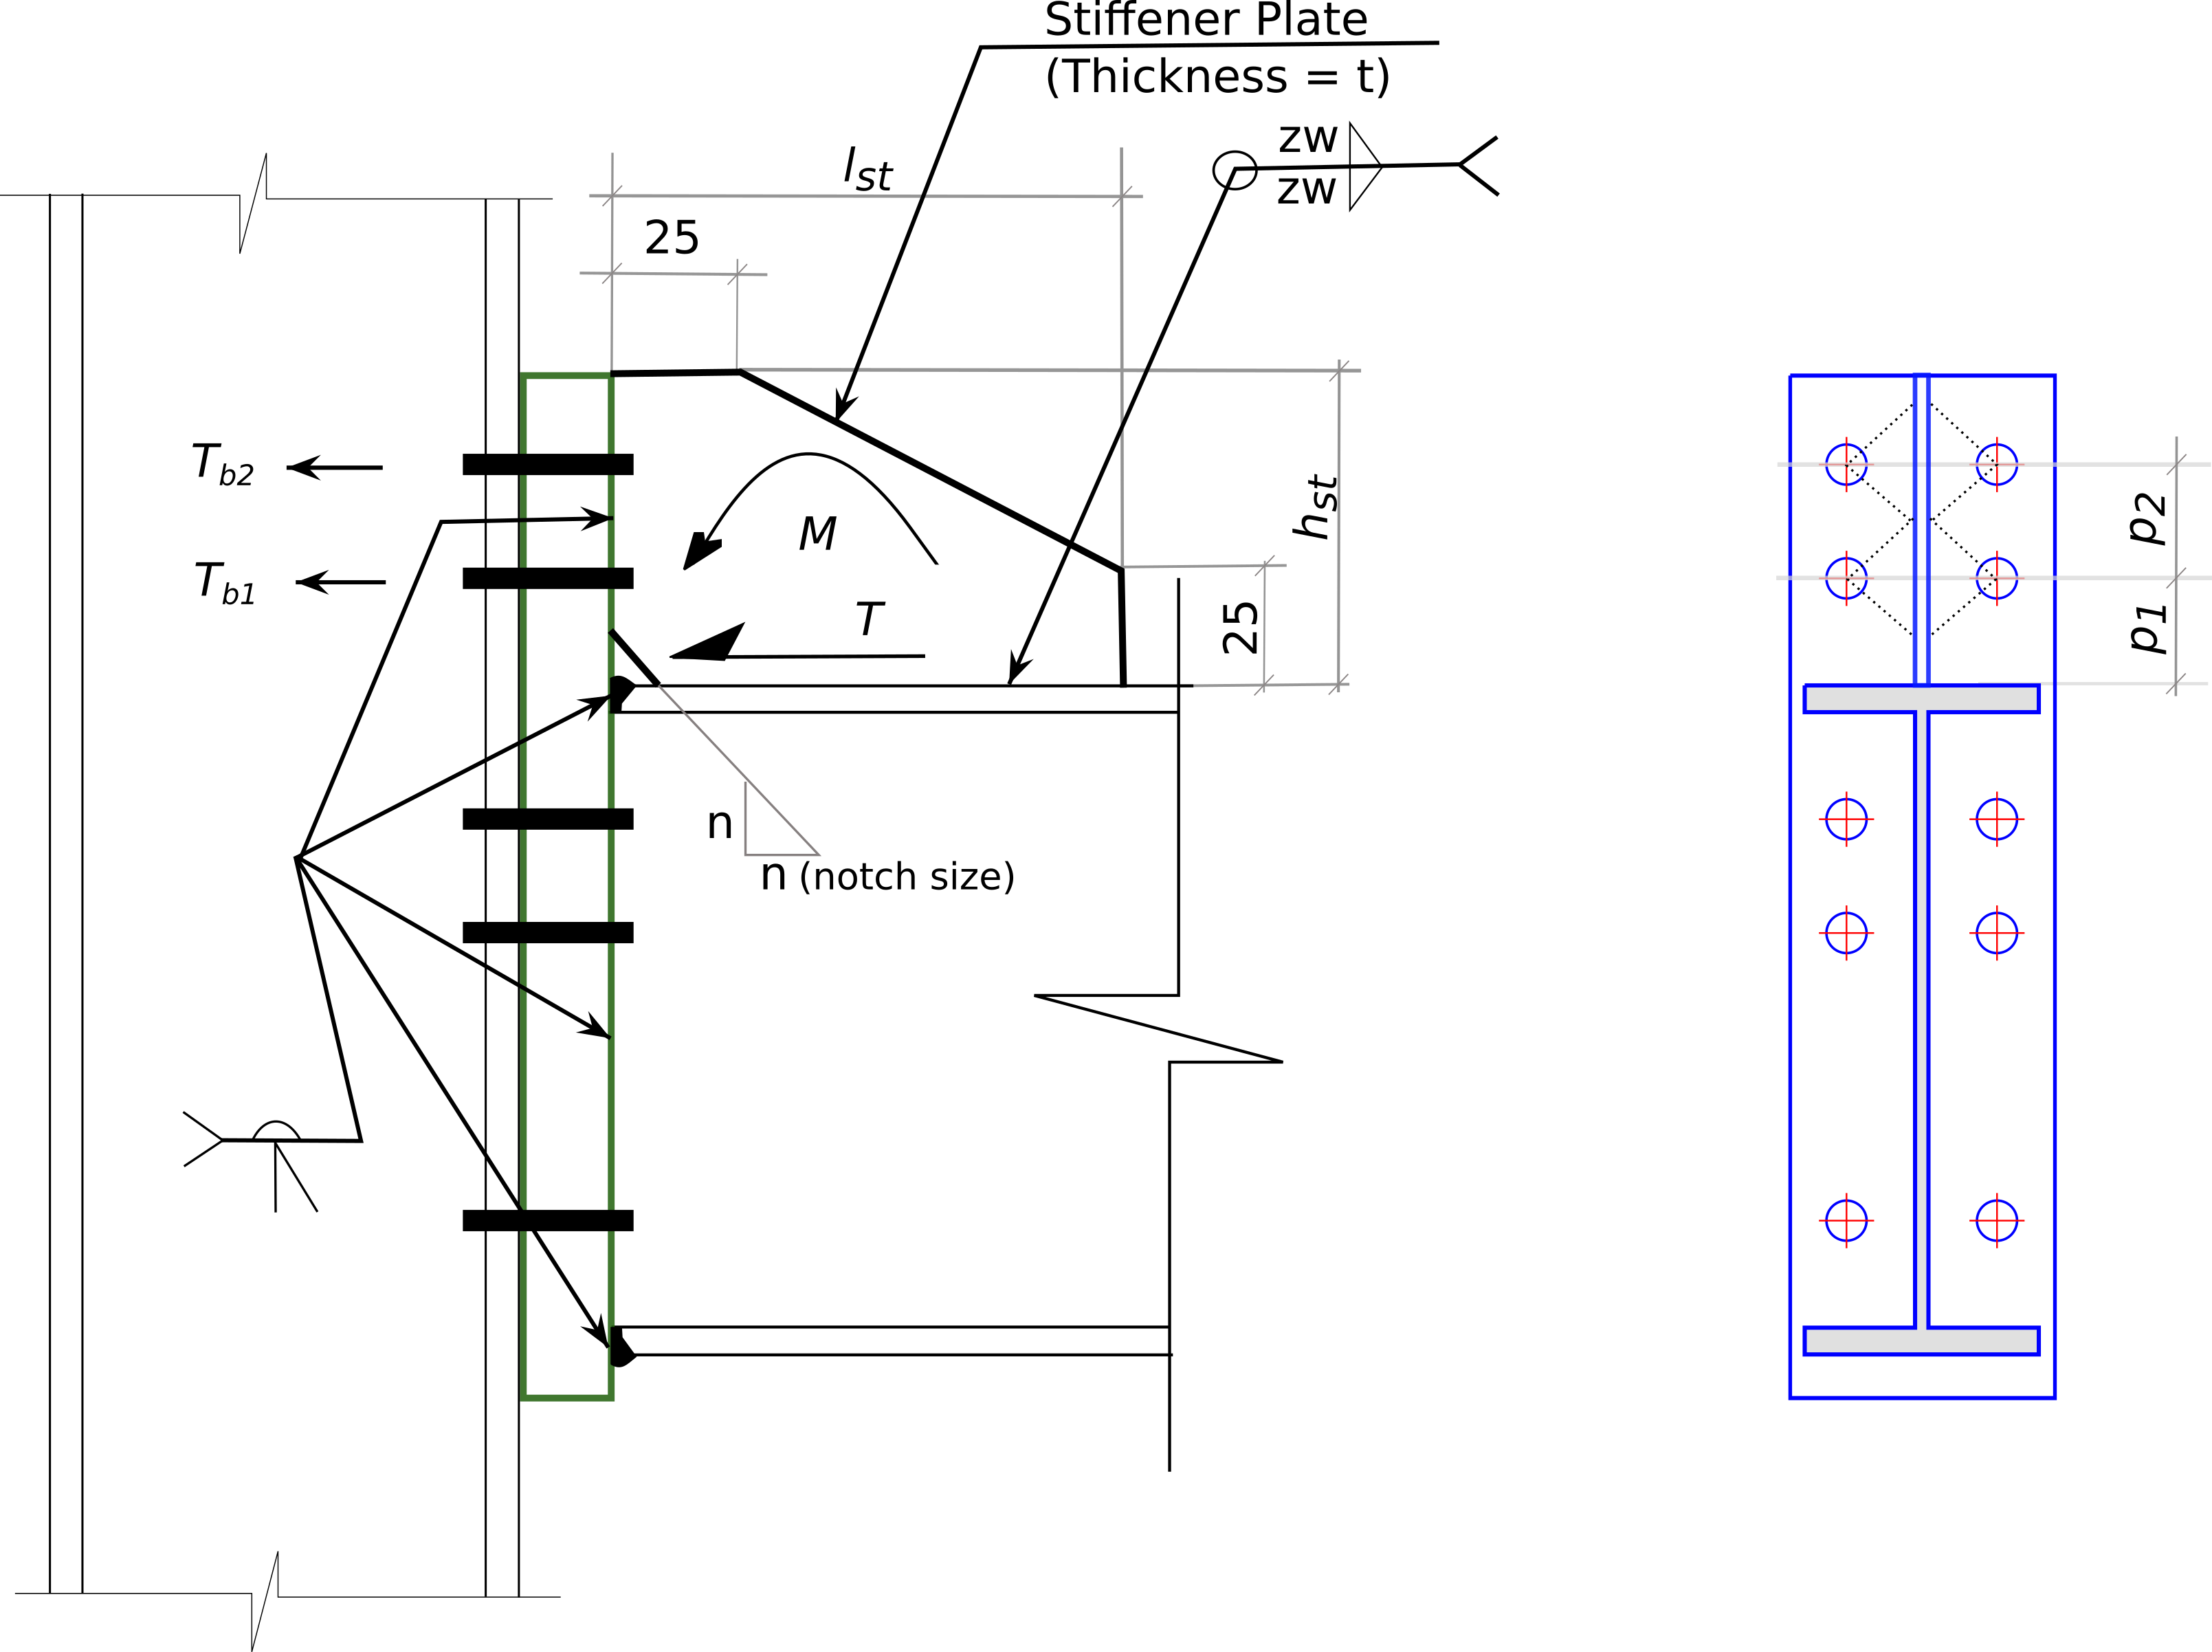
\includegraphics[scale=0.5]{EPStiffeners.png}
\begin{figure}[htp]
	\centering
	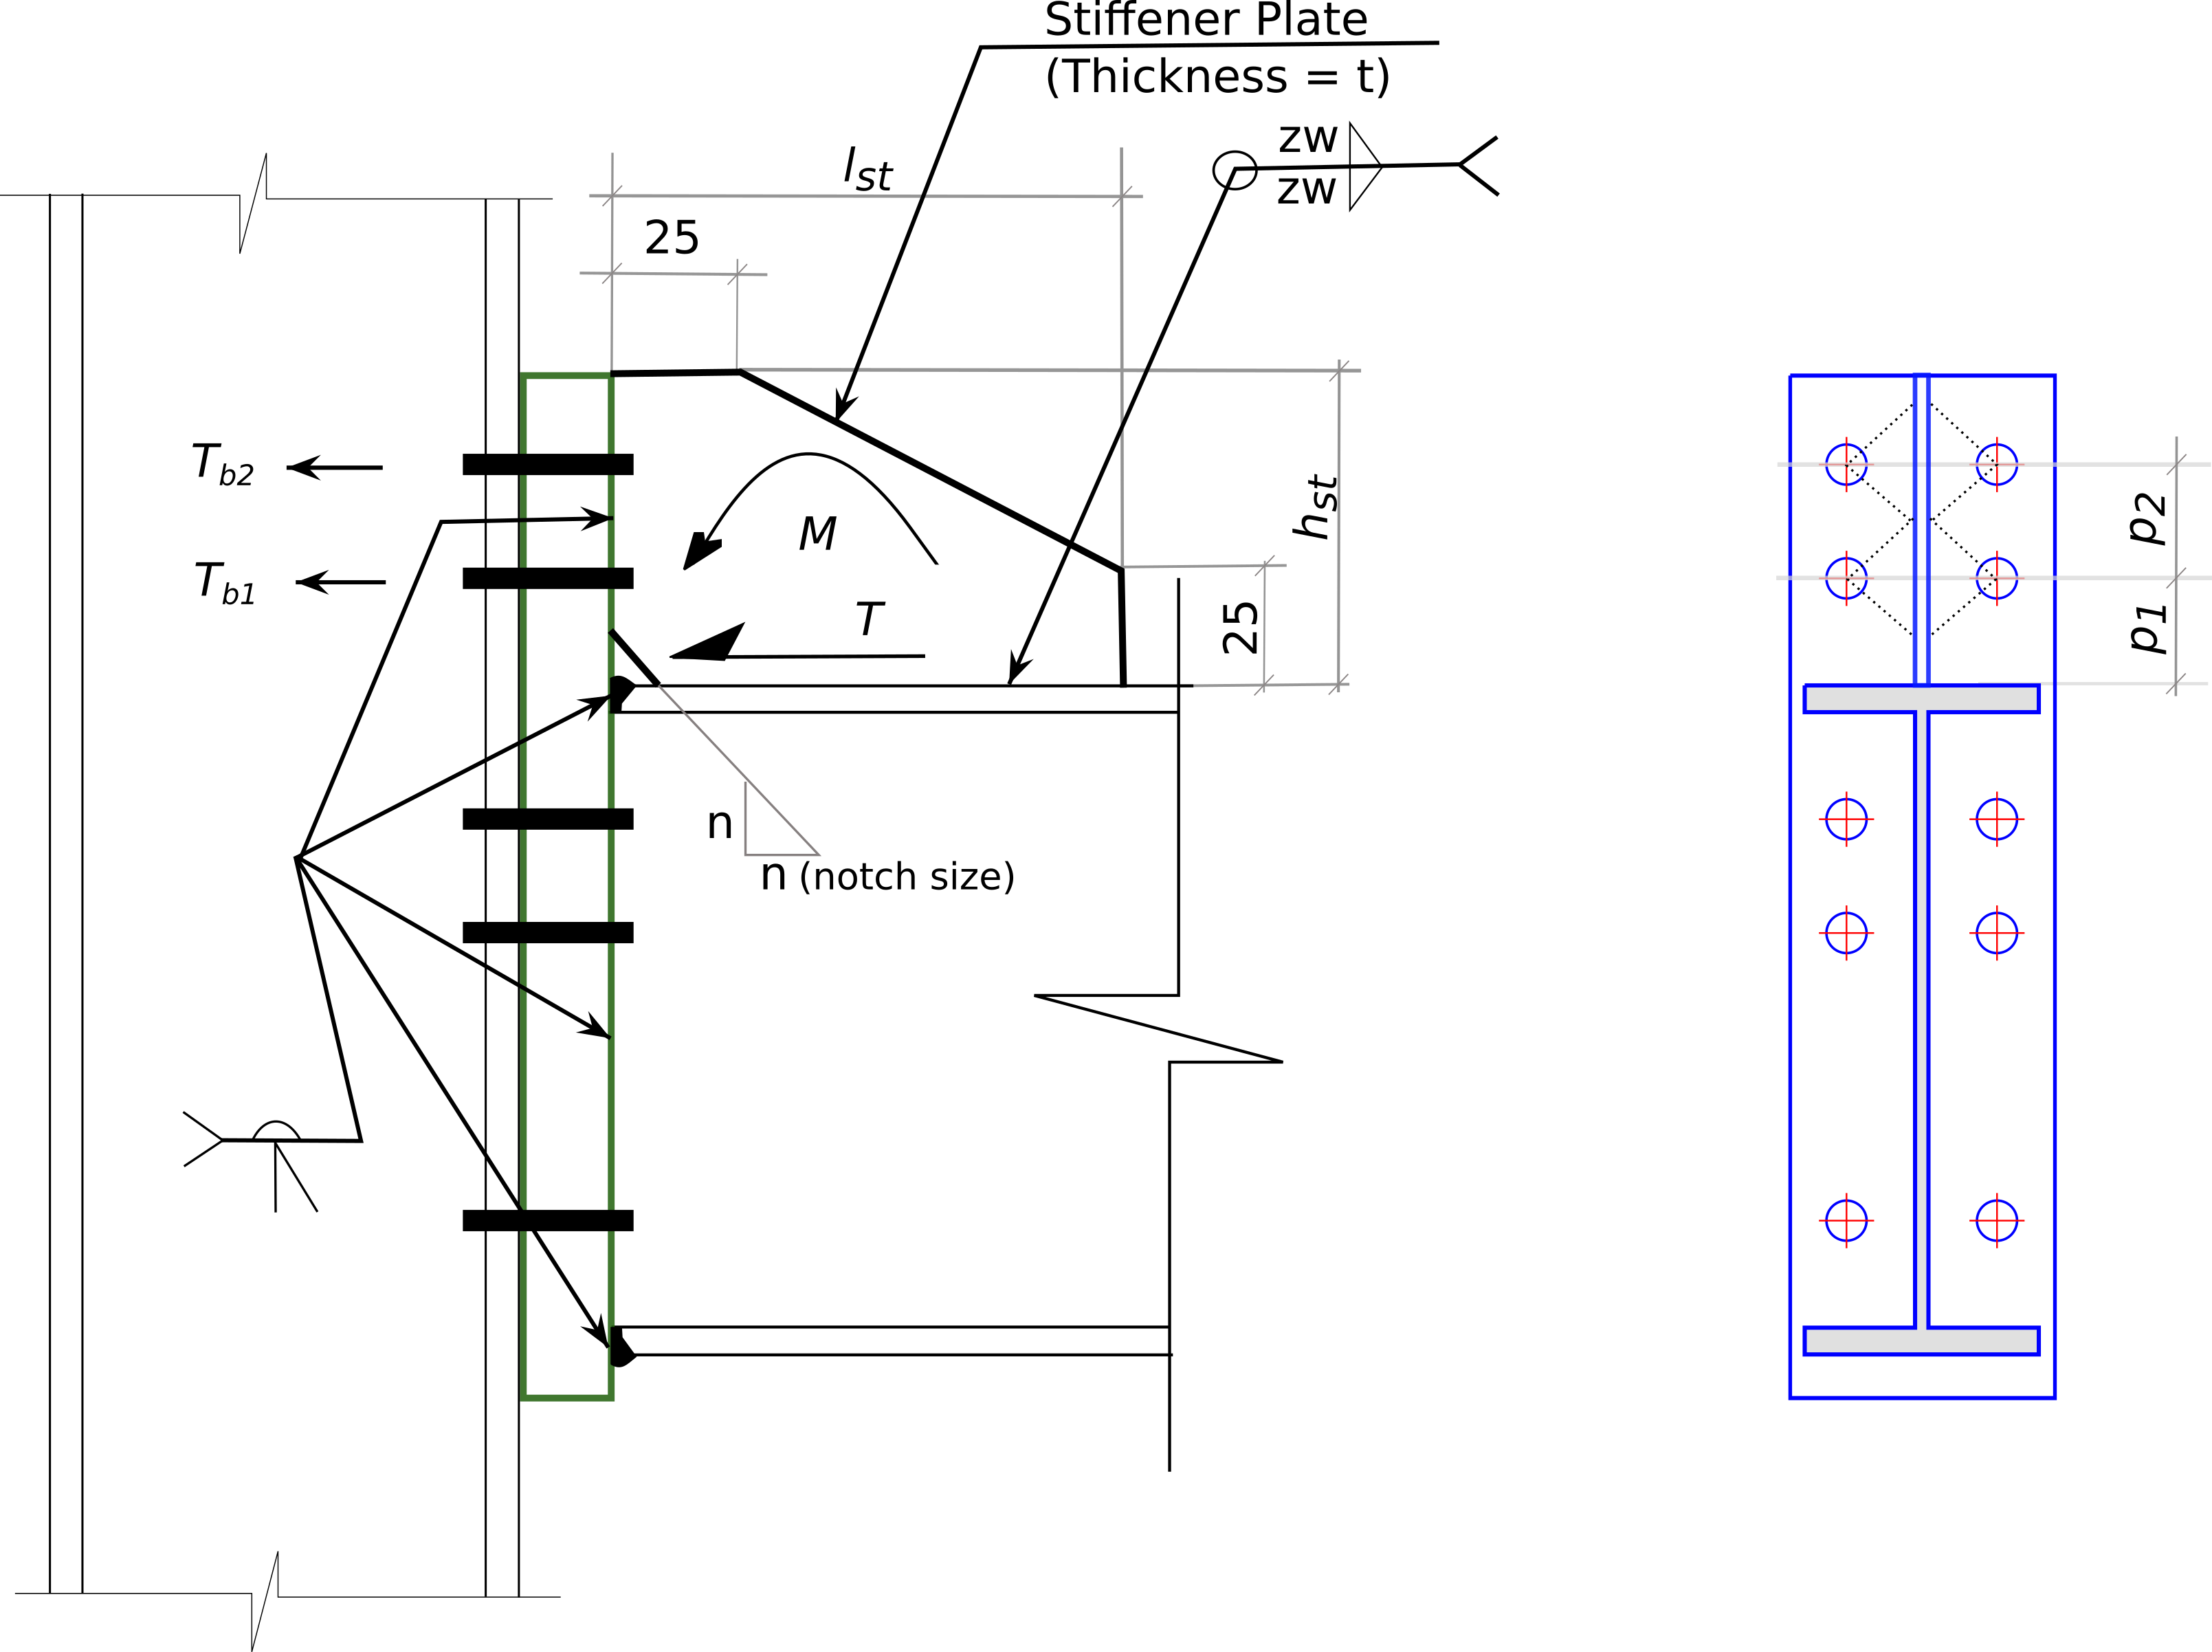
\includegraphics[scale=0.5]{EPStiffeners.png}
	%\caption{}
	%\label{fig:EPstiffener}
\end{figure}



\noindent
Total force transferred to the stiffener, $P_{st}$ = 2x ($T_{b1} + T_{b2}$)\\
%considering that full force in the bolts will be transferred to the stiffener rather than the beam flange.
C.G. of the bolts, $e$ = ($P_1 + P_2/2$)\\
Induced moment in the stiffener, $M_{st} = P_{st}.e$\\
\\
\indent $T_{bi}$ = bolt force in the $i^{th}$ row \\
\indent $P_i$ = pitch of the $i^{th}$ row of bolt\\
\\
\subsection{Check of the stiffener plate}
Effective length of the stiffener, $l_{st,eff} = l_{st} - n$\\
\\
Shear capacity of the stiffener plate, $V_{st} = \frac{l_{st,eff} t_{st} . f_y}{\sqrt{3} \gamma_{m0}}$\\
\\
Moment capacity of the stiffener plate $M_{st} = \frac{l_{st,eff}^2 t_{st} . f_y}{4 \gamma_{m0}}$\\
\\

\subsection{Check for stiffener weld}
Effective length of the weld available, $l_w = (l_{eff} - 2.w)$\\
\\
Shear capacity of the weld, $V_w = \frac{2. l_w w_{tt} . f_u}{\sqrt{3} \gamma_{mw}}$\\
\\

\subsubsection{Combined check of weld for bending and shear stress}
Developed shear stress, $q = \frac{P_{st}}{2.l_w.s_{tt}}$\\
\\
Developed normal stress due to induced bending moment, $f_a = \frac{ M_{st}}{2.(w_{tt}.l_w^2/4)}$\\
\\
So, equivalent stress, 
%Referece can also be drawn to Cl 4.5.3 of EN 1993-1-8 : 2005
%Two methods have been suggested, Directional Method and Simplified Method
%In IS 800, these two have been combined and hence the check is on too much conservative side.
\begin{equation}
	f_e = \sqrt{f_a^2 + q^2}
\end{equation}
\\
As per cl 10.5.10.1.1 of IS 800:2007, check, 
\begin{equation}
	f_e \leq \frac{f_u}{\sqrt{3} \gamma_{mw}}
\end{equation}


%------------------------------------------------------
%------------------------------------------------------
\end{Form}
\end{document}

